\documentclass[12pt,a4paper]{article}
\usepackage[utf8]{inputenc}
\usepackage[american]{babel}
\usepackage{amsmath}
\usepackage{amsfonts}
\usepackage{amssymb}
\usepackage{mathtools}
\DeclarePairedDelimiter{\abs}{\lvert}{\rvert}
\newcommand{\pdiff}[2]{\frac{\partial #1}{\partial #2}}
\newcommand{\pdiffn}[3]{\frac{\partial^{#3} #1}{\partial #2^{#3}}}
\usepackage{geometry}
\usepackage[square]{natbib}
\usepackage[bookmarks,hidelinks]{hyperref}
\usepackage{subfiles}
\usepackage[numbib,nottoc]{tocbibind}
\usepackage{url}
\usepackage{siunitx}
\usepackage{listings}
\usepackage{color}
\lstset{
  language=Python,
  keywordstyle=\bfseries\ttfamily\color[rgb]{0,0,1},
  identifierstyle=\ttfamily,
  commentstyle=\color[rgb]{0.133,0.545,0.133},
  stringstyle=\ttfamily\color[rgb]{0.627,0.126,0.941},
  showstringspaces=false,
  basicstyle=\small,
  numberstyle=\footnotesize,
  numbers=left,
  stepnumber=5,
  numberfirstline=true,
  breaklines=true,
  breakatwhitespace=false,
  frame=single
}
\usepackage{tikz}
\usetikzlibrary{patterns}
\renewcommand{\epsilon}{\varepsilon}
\usepackage{titling}
\newcommand{\subtitle}[1]{
  \posttitle{
    \par\end{center}
    \begin{center}\large#1\end{center}
    \vskip0.5em}
}
\author{Marc John Bordier Dam}
\title{Using Numerical Methods to Explore Quantum Mechanics}
\linespread{1.3}

\begin{document}
\selectlanguage{american}
\maketitle

\begin{abstract}
This report uses numerics to study a Gaussian wave package in an infinite square well and in a finite square well inside an infinite square well. We find that the wave package loses its shape over time although it returns to its initial state eventually and shows periodic behavior.
\end{abstract}

\tableofcontents

\section{Introduction}
In this report we will study two different potentials: The infinite square well and the finite square well inside an infinite square well. The infinite square well corresponds to a particle trapped in a box and is an idealized model of an electron trapped in a long organic molecule e.g. $\beta$-carotene. The finite square well is interesting to study since it is possible to find a bound particle outside the well. This differs from the classical behavior where a bound particle can only be found inside the well. The finite square well potential is shown in figure~\ref{fig:finiteSquareWell}. For a figure of the infinite square well just imagine figure~\ref{fig:finiteSquareWell} with inifinitely tall walls.

\section{Schrödinger's Equation and its Solutions}
The most fundamental equation in quantum mechanics is the Schrödinger equation. It governs which functions are worthy of study, that is, which functions are allowed wave functions in a given potential. The time-dependent Schrödinger equation in one dimension is
\begin{equation}
i \hbar \pdiff{\Psi}{t} = - \frac{\hbar^2}{2 m} \pdiffn{\Psi}{x}{2} + V \Psi.
\end{equation}
To make solving the time-dependent Schrödinger equation easier we use separation of variables to obtain the time-independent Schrödinger equation
\begin{equation}
- \frac{\hbar^2}{2 m} \pdiffn{\psi}{x}{2} + V \psi = E \psi,
\end{equation}
where $\Psi = \psi e^{-\frac{i E t}{\hbar}}$.

The wave functions which are solutions to the time-independent Schrödinger euqation represent stationary states. These stationary states have the nice property that any function in Hilbert space can be written as a linear combination of them. Thus it is in many cases sufficient to work with the stationary states and linear combinations of them. Below we will present the stationary states along with their allowed energies for the infinite and finite square well.

\subsection{The Infinite Square Well}
\begin{figure}
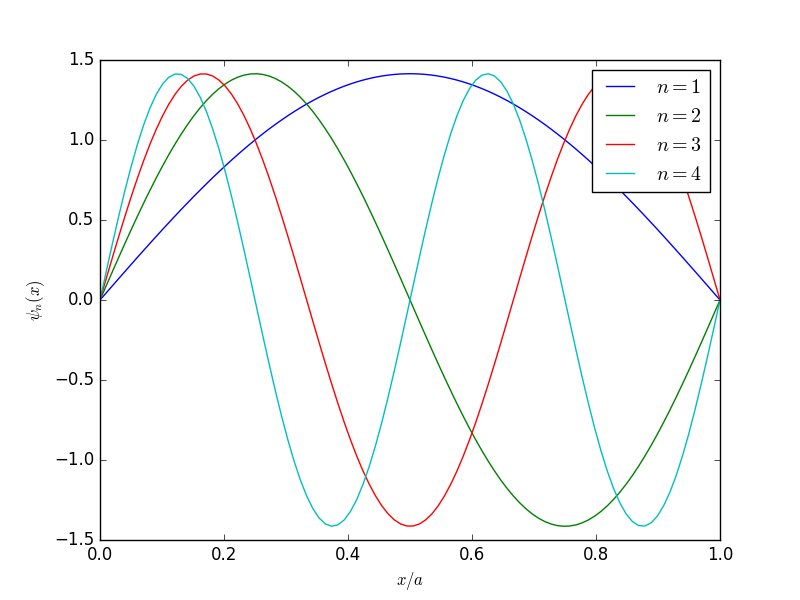
\includegraphics[width=\textwidth]{../Python/ISW_stationarySolutions.png}
\caption{Wave Functions in the Infinite Square well}
\label{fig:infiniteSquareWell}
\end{figure}

In the infinite square well the potential is given by
\begin{equation}
V = \begin{cases} 0, & 0 \leq x \leq a \\
                  \infty, & \text{otherwise} \end{cases}.
\end{equation}

Outside the well the wave function is $0$ and inside the well it is given by
\begin{equation}
\psi_n(x) = \sqrt{\frac{2}{a}} \sin \left( \frac{n \pi}{a} x \right),
\end{equation}
where $n$ is any positive integer. In the infinite square well the energy spectrum is discrete with the $n$th stationary state having the energy
\begin{equation}
E_n = \frac{n^2 \pi^2 \hbar^2}{2 m a^2}.
\end{equation}
Some of the wave functions are shown in figure~\ref{fig:infiniteSquareWell}.

\subsection{The Finite Square Well}
\begin{figure}
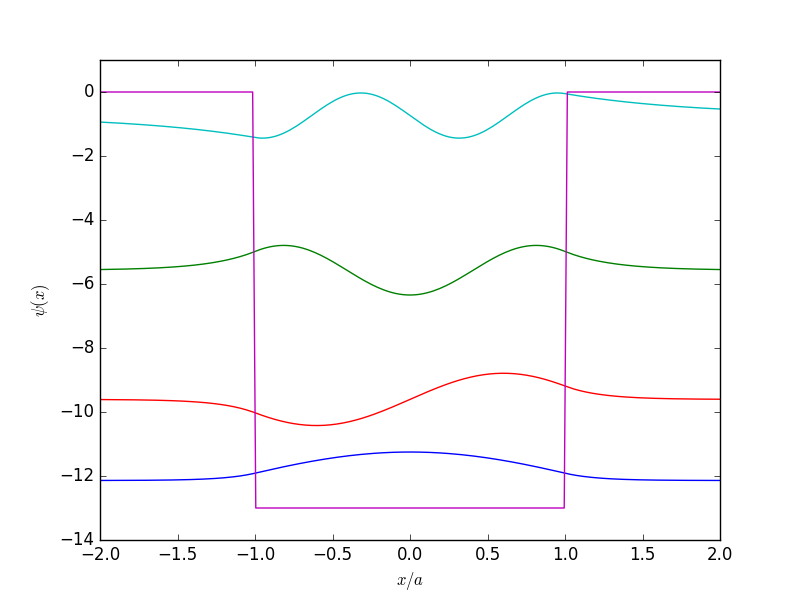
\includegraphics[width=\textwidth]{../Python/FSW_boundStates.png}
\caption{Wave Functions in the Finite Square well}
\label{fig:finiteSquareWell}
\end{figure}

In the finite square well the potential is given by
\begin{equation}
V = \begin{cases} -V_0, & -a \leq x \leq a \\
                  0, & \text{otherwise} \end{cases},
\end{equation}
where $V_0$ is a positive number.

In the finite square well the wave function can be found both inside and outside the well. We also have both bound ($E < 0$) and scattering states ($E > 0$) in the finite square well.

The bound states come in two flavors: Even and odd. The even wave functions are given by
\begin{equation}
\psi_{even} (x) = \begin{cases} A e^{- \kappa x}, & a < x \\
                                A \frac{e^{- \kappa a}}{\cos la} \cos l x, & -a \leq x \leq a \\
                                A e^{\kappa x}, & x < -a \end{cases},
\end{equation}
where $A$ is a normalization constant, $\kappa = \frac{\sqrt{-2 m E}}{\hbar}$ and $l = \frac{\sqrt{2 m (E + V_0)}}{\hbar}$.

Similarly the odd wave functions are given by
\begin{equation}
\psi_{odd} (x) = \begin{cases} A e^{- \kappa x}, & a < x \\
                                A \frac{e^{- \kappa a}}{\sin la} \sin l x, & -a \leq x \leq a \\
                                - A e^{\kappa x}, & x < -a \end{cases},
\end{equation}
where again $A$ is a normalization constant, $\kappa = \frac{\sqrt{-2 m E}}{\hbar}$ and $l = \frac{\sqrt{2 m (E + V_0)}}{\hbar}$.

The energy spectrum of the bound states is discrete but can not be determined analytically. Defining $z = l a$ and $z_0 = \frac{a}{\hbar} \sqrt{2 m V_0}$ the allowed energies for the even wave functions can be found by solving the equation
\begin{equation}
\tan z = \sqrt{\left(\frac{z_0}{z} \right)^2 - 1}. \label{eq:evenEnergy}
\end{equation}
Likewise the allowed energies for the odd wave functions can be found by solving the equation
\begin{equation}
- \cot z = \sqrt{\left(\frac{z_0}{z} \right)^2 - 1}. \label{eq:oddEnergy}
\end{equation}
Some of the wave functions for the bound states are shown in figure~\ref{fig:finiteSquareWell}.

The wave functions for the scattering states are given by
\begin{equation}
\psi(x) = \begin{cases} F e^{ikx} & a < x \\
                        C \sin lx + D \cos lx & -a \leq x \leq a \\
                        A e^{ikx} + B e^{-ikx} & x < -a \end{cases},
\end{equation}
where $A$ is a normalization constant and
\begin{align*}
k &= \frac{\sqrt{2 m E}}{\hbar}, \\
l &= \frac{\sqrt{2 m (E + V_0)}}{\hbar}, \\
B &= i \frac{\sin 2 la}{2 kl} \left( l^2 - k^2 \right) F, \\
C &= \left( \sin la + i \frac{k}{l} \cos la \right) e^{ika} F, \\
D &= \left( \cos la - i \frac{k}{l} \sin la \right) e^{ika} F, \\
F &= \frac{e^{-2ika}}{\cos 2la - i \frac{k^2 + l^2}{2kl} \sin 2la} A.
\end{align*}
For the scattering states we observe reflection and transmission through the well wall.

The energy spectrum of the scattering states is continuous and thus any positive energy is allowed.

\section{Quantum Mechanics in Reduced Units}
When doing simulations we want to work with the physical quantities in reduced units. We do this for two reasons: We don't have to keep track of the units on everything and quantities in reduced units tend to be of a reasonable order of magnitude.

In our simulations we have three constants: The particle mass $m_0$, the well width $a$ and Planck's constant $\hbar$. In our system of reduced units these will all be equal to $1$. With these three constants we can derive the reduced units for the remaining relevant quantities in our simulation. The relevant quantities are shown in table~\ref{tab:reducedUnits}, where the real values for an electron in a $\pi$-bond in an ethylene molecule is also shown.

\begin{table}
\caption{Reduced Units (subscript $r$ denotes the quantity in real units)}
\label{tab:reducedUnits}
\begin{tabular}{c|ccc}
Quantity (Q.) & Q. in R. U. & Characteristic Q. & Electron in $\pi$-bond \\ 
\hline 
Length, $x$ & $\frac{x_r}{a}$ & $a$ & $\SI{1,34}{\angstrom}$ \\ 
Mass, $m$ & $\frac{m_r}{m_0}$ & $m_0$ & $m_e = \SI{9,109e-31}{\kilo\gram}$ \\ 
Time, $t$ & $\frac{t_r}{t_0}$ & $t_0 = \frac{m_0 a^2}{\hbar}$ & $\SI{1,55e-16}{\second}$ \\ 
Energy, $E$ & $\frac{E_r}{E_0}$ & $E_0 = \frac{\hbar^2}{m_0 a^2}$ & $\SI{6,80e-19}{\joule}$ \\ 
Velocity, $v$ & $\frac{v_r}{v_0}$ & $v_0 = \frac{\hbar}{m_0 a}$ & $\SI{8,64e5}{\meter\per\second}$ \\ 
Momentum, $p$ & $\frac{p_r}{p_0}$ & $p_0 = \frac{\hbar}{a}$ & $\SI{7,87e-25}{\meter\kilogram\per\second}$ \\ 
\end{tabular} 
\end{table}

\subsection{Schrödinger's Equation in Reduced Units}
Since $m$ and $\hbar$ both are equal to $1$ in our system of reduced units the time-dependent Schrödinger equation takes the form
\begin{equation}
i \pdiff{\Psi}{t} = - \frac{1}{2} \pdiffn{\Psi}{x}{2} + V \Psi,
\end{equation}
where $t$, $x$ and $V$ are all in reduced units. Likewise the time-indepedent Schrödinger equation takes the form
\begin{equation}
- \frac{1}{2} \pdiffn{\psi}{x}{2} + V \psi = E \psi,
\end{equation}
where again $x$, $V$ and $E$ are all in reduced units and $\Psi = \psi e^{i E t}$. The stationary wave functions in the infinite square well along with the allowed energies take the form
\begin{equation}
\psi_n(x) = \sqrt{2} \sin (n \pi x), \quad E_n = \frac{n^2 \pi^2}{2}.
\end{equation}
The wave functions representing bound stationary states take the form
\begin{equation}
\psi_{even}(x) = \begin{cases} A e^{-\sqrt{-2 E} x}, & 1 < x \\
                               A \frac{e^{-\sqrt{-2 E}}}{\cos \sqrt{2(E + V_0)}} \cos \left( \sqrt{2(E + V_0)} x \right), & -1 \leq x \leq 1 \\
                               A e^{\sqrt{-2 E} x}, & x < -1 \end{cases}
\end{equation}
and
\begin{equation}
\psi_{odd}(x) = \begin{cases} A e^{-\sqrt{-2 E} x}, & 1 < x \\
                              A \frac{e^{-\sqrt{-2 E}}}{\sin \sqrt{2(E + V_0)}} \sin \left( \sqrt{2(E + V_0)} x \right), & -1 \leq x \leq 1 \\
                              -A e^{\sqrt{-2 E} x}, & x < -1 \end{cases}.
\end{equation}
These equations along with equation~\eqref{eq:evenEnergy} and equation~\eqref{eq:oddEnergy} in reduced units is what will form the basis of our numerical investigations of the infinite and finite square well.

An idealized model of the $\pi$-bond in an ethylene molecule is an infinite square well where the width of the well is the length of a bond. The particle confined in the well then corresponds to an electron confined in a $\pi$-bond. The bond length between the two carbon atoms in ethylene is about $\SI{1.34}{\angstrom}$ and the mass of the electron is about $m_e = \SI{9.109e-31}{\kilo\gram}$. Using these numbers we can make a conversion table (table~\ref{tab:reducedUnits}) which allows us to convert from reduced units in our simulation to the real world example of an electron in a $\pi$-bond in an ethylene molecule.

\section{Numerics}
In this section we will introduce the software as well as some of the numerical methods we have used in the process of simulation the potentials and wave packages.

\subsection{The Tools}
In this project we have used Python to numerically simulate a guassian wave package in an infinite square well and in a finite square well inside an infinite square well.

Since Python does not have native support for working with matrices we have used the NumPy package. NumPy includes tools for working with matrices and multidimensional arrays as well as tools for doing numerical integration and differentiation.

The function \lstinline{numpy.trapz} does numerical integration with the trapezoidal method which approximates the area under a curve using trapezoids. The function \lstinline{numpy.gradient} does numerical differentiation using a finite difference method.

For plotting we have used the Matplotlib package. We have also used the Matplotlib package for producing the animated videos of the plots.

\subsection{Root Finding}
When working with the finite square well we need to do numerical root finding to determine the allowed energies. We use Newton's method to determine the solutions to equation~\eqref{eq:evenEnergy} and equation~\eqref{eq:oddEnergy}.

Newton's method works by repeatedly estimating the root using a linear approximation of the function we wish to find the root of. As always we use a first order Taylor expansion to find a linear approximation. Starting from an initial guess of $x_0$ this gives us the equation
\begin{equation}
0 = f(x_0) + f'(x_0)(x - x_0)
\end{equation}
If we solve for $x$ we get that
\begin{equation}
x = x_0 - \frac{f(x_0)}{f'(x_0)}. \label{eq:newtonNonRecurring}
\end{equation}
Since we arrived at this ``root'' by using an approximation we would expect that this ``root'' is also only an an approximation to the real root which we are interested in. Since linear approximations of differentiable functions are more accurate the closer we are to the point around which we approximate, we can get a better estimate of our root by repeating the process. Thus we rewrite equation~\eqref{eq:newtonNonRecurring} as a recurrence relation
\begin{equation}
x_{n+1} = x_n - \frac{f(x_n)}{f'(x_n)}.
\end{equation}
For the implementation used in our script see the appendix~\ref{app:newton}.

\subsection{Code Structure}
The code for each potential is divided into a number of modules. The lowest level module \verb!psi_n! (named \path{psi_n.py}, \path{FSW_psi_n_bound.py} and \path{WiW_psi_n.py} respectively) contains the wave functions of the time-independent stationary states as well as the energies corresponding to the stationary states. It takes the wave function index $n$ as well as a position array as arguments.

The \verb!psi_n! module is then used in the \verb!Psi_n! module (named \path{Psi_n.py}, \path{FSW_Psi_n_bound.py} and \path{WiW_Psi_n.py} respectively) which contains the time-depedent wave functions. This module takes a time value as argument in addition to the arguments of the \verb!psi! module.  The \verb!Psi_n! module is then used to construct the general wave function. This is done in the \verb!Psi! module (named \path{Psi.py}, \path{FSW_Psi_bound.py} and \path{WiW_Psi.py} respectively) which takes a list of coefficients $c_n$ as an argument in addition to the arguments of the \verb!Psi_n! module.

To get the $c_n$'s for an arbitrary wave function we use Fourier's trick to get the projection of the wave function on the stationary states. This is done in the module \verb!getcn! (named \path{getcn.py}, \path{FSW_getcn_bound.py} and \path{WiW_getcn.py} respectively) which determines the $c_n$'s by numerical integration. The \verb!getcn! module has two different options. It can either determine a fixed number of $c_n$'s or determine enough $c_n$'s to make the sum of the norm squares within an $\epsilon$ of $1$. In the case of the bound states in the finite square well it is not always possible to ensure that the $c_n$'s have the required norm since there is a finite number of bound states in the finite square well.

We gather all these in the main script (named \path{wavePackageSimultaneousPlot.py} and \path{WiW_wavePackageSimultaneousPlot.py} respectively) where we simulate the wave package in the potential.	The overall structure of the script is to first load in the modules \verb!Psi! and \verb!getcn!. Then we define and normalize the wave package. After this we use the \verb!getcn! module to get a list of $c_n$'s which we then use to calculate the linear combination of stationary states using the \verb!Psi! module. With the setup done we then calculates $\langle x \rangle$, $\langle x^2 \rangle$, $\langle p \rangle$ and $\langle p^2 \rangle$ using \lstinline{numpy.trapz} and \lstinline{numpy.gradient}. These values can be used to calculate $\sigma_x$ and $\sigma_p$ which we use to check that the uncertainty principle holds. Finally we calculate the momentum distribution by projecting the wave function $\Psi$ onto the eigenfunctions of the momentum operator. The remainder of the script is used to animate the wave package along with its momentum spectrum.

\section{Numerical Results}
In this section we present the numerical results obtained from simulating a wave package in the infinite square well and in the finite square well inside an infinite square well.

The infinite square well extends from $0$ to $1$ in reduced units. The finite square well inside the infinite square well is made such that the finite square well extends from $-1$ to $1$ in reduced units and the surrounding infinite square well extends from $-3$ to $3$ in reduced units.

We have simulated a Gaussian wave package given by the equation
\begin{equation}
\Psi(x, 0) = A e^{- \frac{1}{2} \frac{(x - x_0)^2}{\sigma_0^2}} e^{- i k_0 x},
\end{equation}
where $A$ is a normalization constant. In the infinite square well we set $x_0 = 0.5$, $\sigma_0 = 0.1$ and $k_0 = 100$. The simulated wave package is a linear combination of the first 48 staionary states. In the finite square well inside an infinite square well we set $x_0 = 2.5$, $\sigma_0 = 0.1$ and $k_0 = 25$. This wave package is a linear combination of the first 110 stationary states. The time evolution as well as the momentum spectrum of these wave packages are shown in the accompanying videos.

\begin{figure}
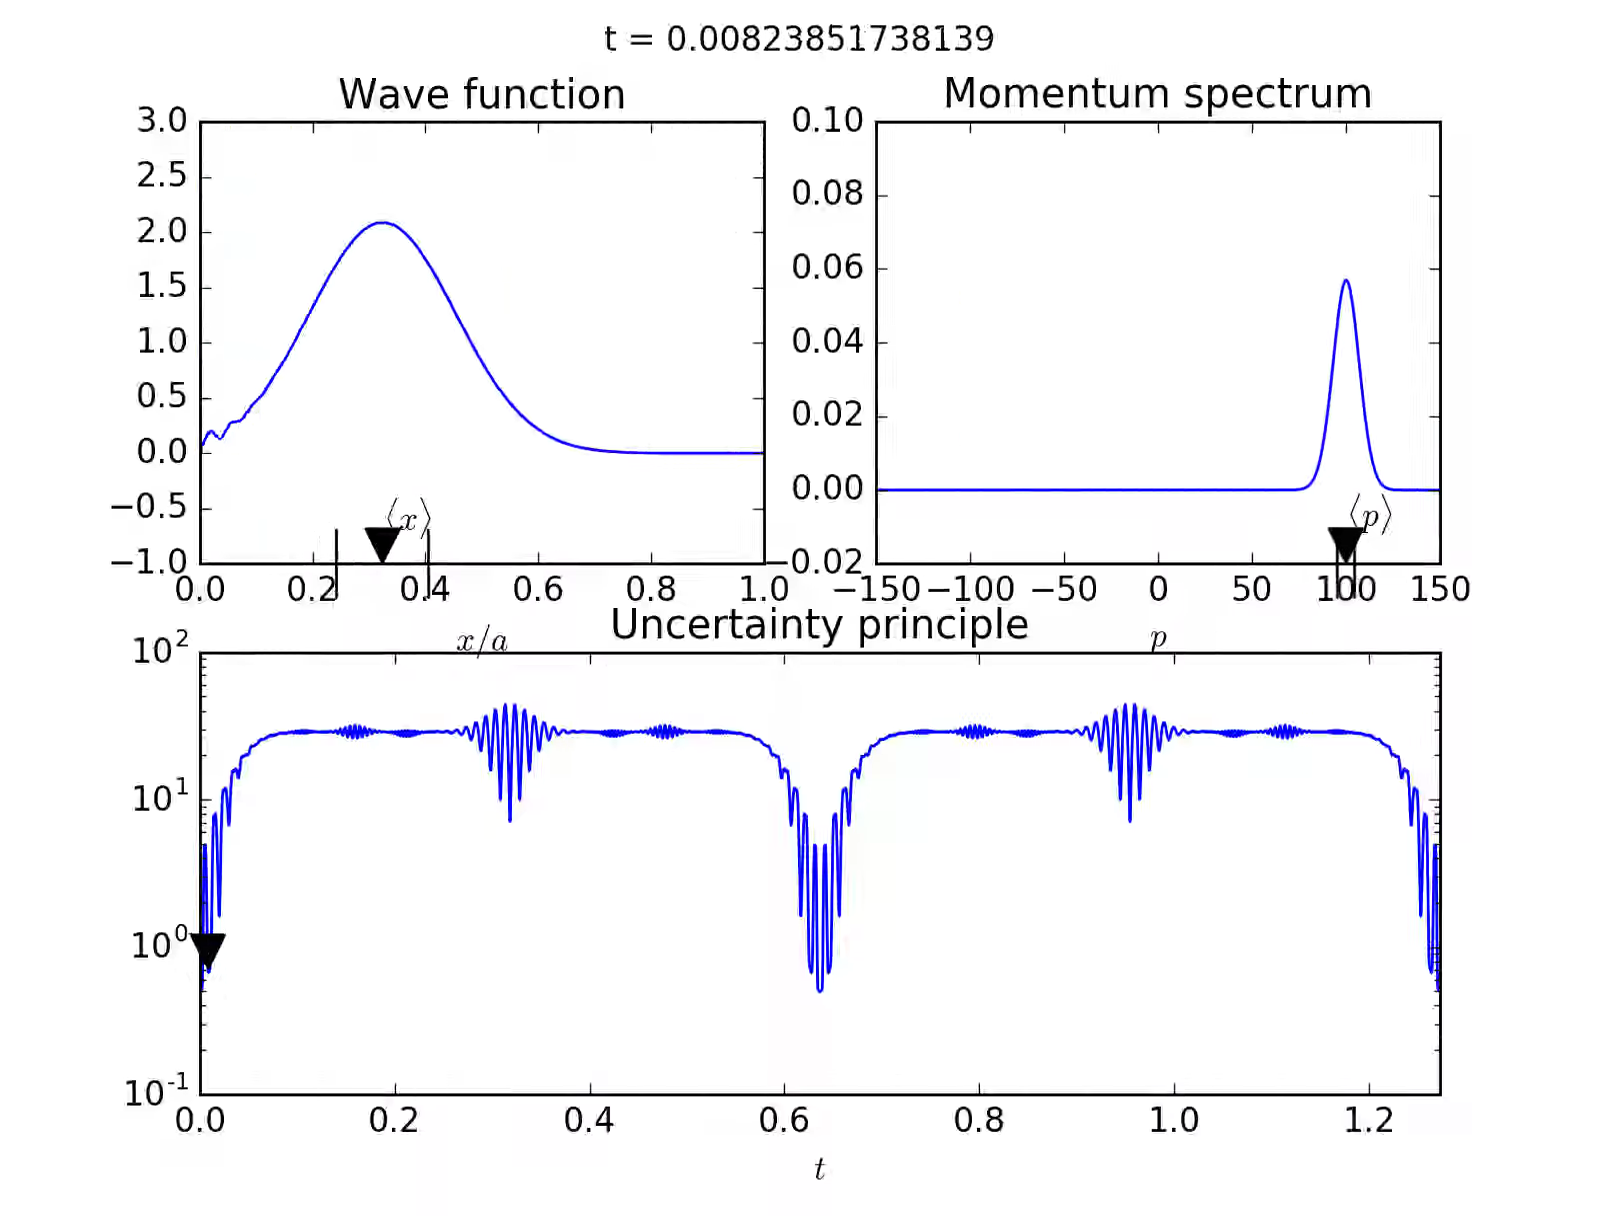
\includegraphics[width=\textwidth]{ISW_wavePackageEarly.png}
\caption{The wave package in the infinite square well along with its momentum spectrum at $t = 0.00823851738139$. The wave package has just bounced off of the left wall and has momentum to the right.} \label{fig:wavePackageInit}
\end{figure}

\begin{figure}
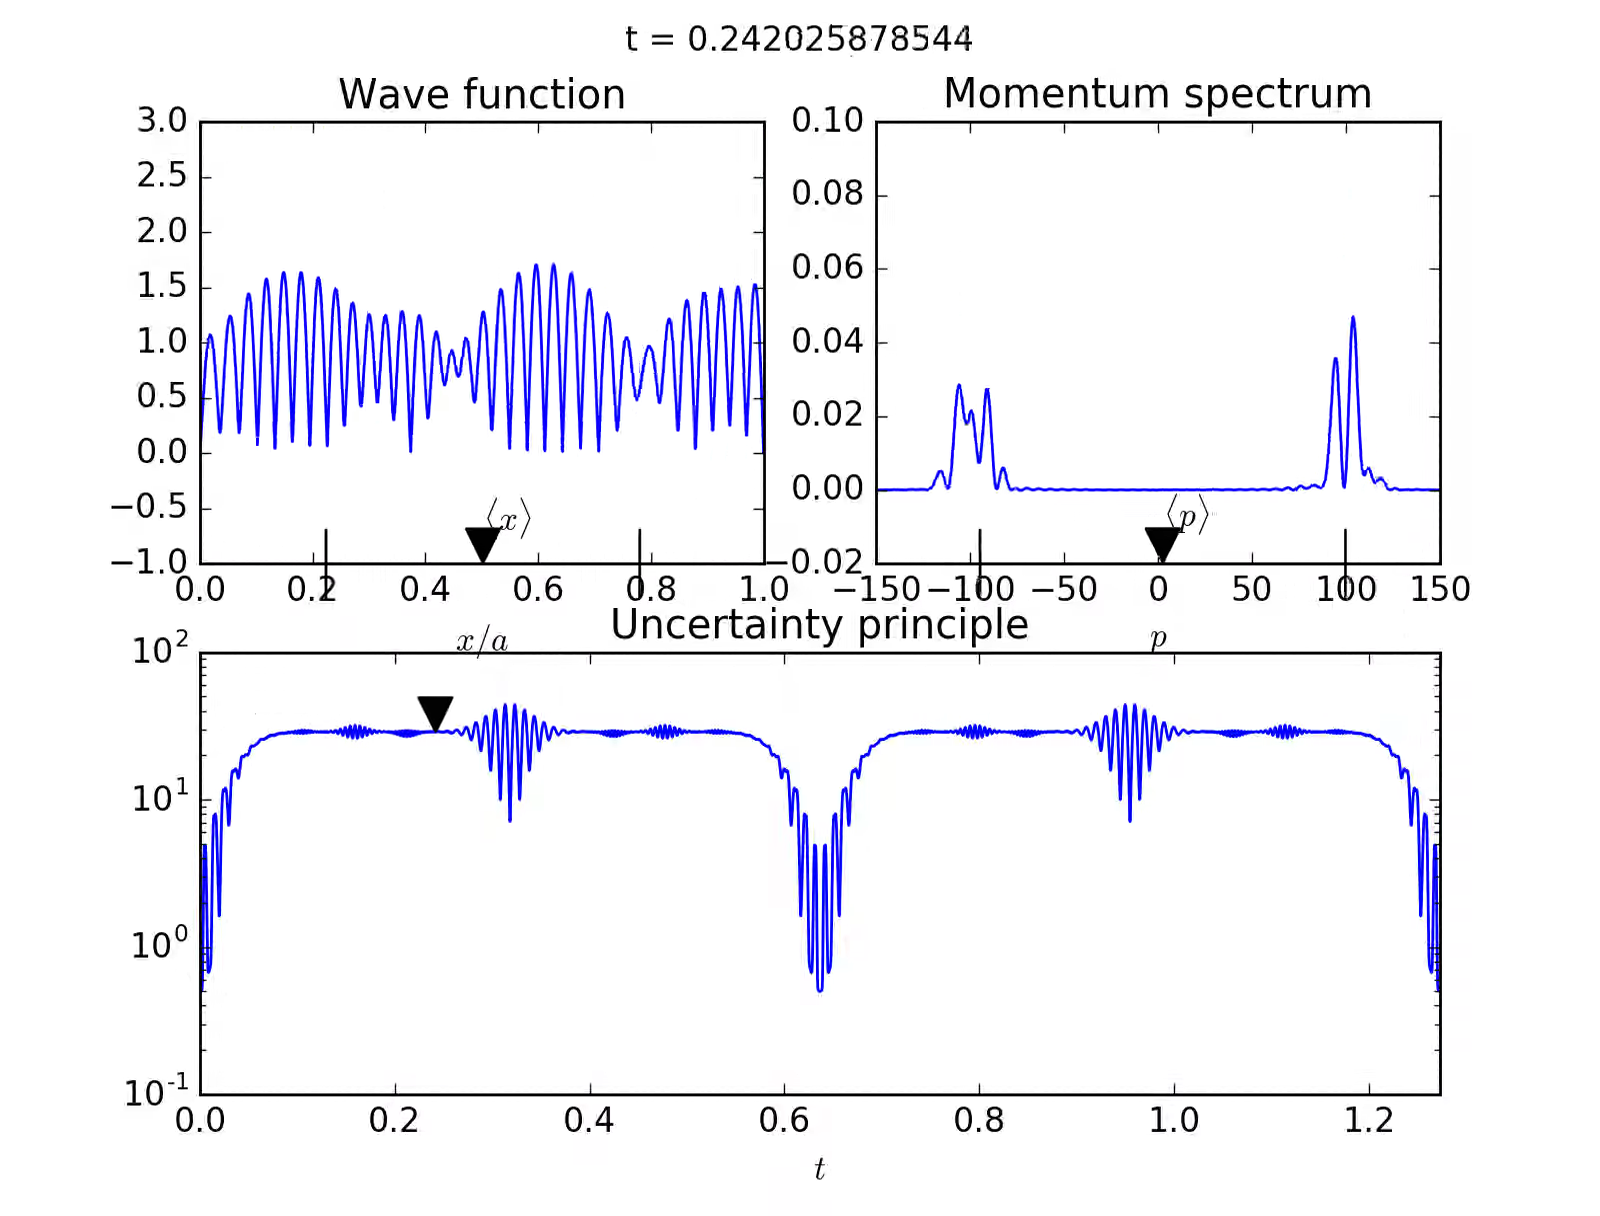
\includegraphics[width=\textwidth]{ISW_wavePackageLater.png}
\caption{The wave package in the infinite square well along with its momentum spectrum at $t = 0.242025878544$.} \label{fig:wavePackageLater}
\end{figure}

Two snapshots of the wave package in the infinite square well at different times are shown in figure~\ref{fig:wavePackageInit} and figure~\ref{fig:wavePackageLater}. From these figures we see that the wave package has a  well defined shape, position and momentum early on. At time zero $\sigma_x \sigma_p$ for the wave package is close to the lower limit of the uncertainty principle. At later times the wave package has a less well defined shape, position and momentum. This is also consistent with $\sigma_x \sigma_p$ being large. The wave package in the finite square well inside the infinite square well shows similar behavior.

Our numerical simulations highlight an interesting feature of the infinite square well: If we wait long enough the wave package will eventually return to its initial shape. This happens in our simulations because we are working with the periodic functions sine and cosine. In the real world we would not be able to have an isolated wave package in an infinite square well. Perturbations and interactions from outside the well would break the periodicity and it would be very unlikely for the wave package to assume its initial shape at later times. We would also expect that a real world wave package would not return to a state of minimal uncertainty.

It is worth noting that the wave package in the finite square well inside the infinite square well loses its shape faster than the wave package in the infinite square well. This is consistent with the fact that the wave package in the finite square well inside an infinite square well has a higher energy than the wave package in the infinite square well. The finite square well appearently also does some work in spreading out the wave package and we can see from the video of the wave package in the finite square well inside the infinite square well that the standard deviation of the position of the wave package increases as the wave package passes over the finite square well.

\begin{figure}
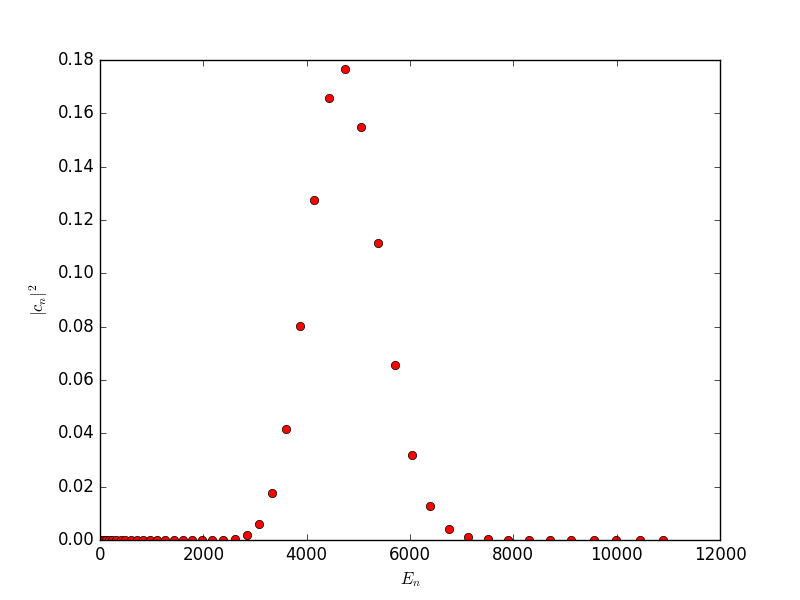
\includegraphics[width=\textwidth]{../Python/ISW_wavePackageEnergySpectrum.png}
\caption{Energy spectrum of the wave package in the infinite square well} \label{fig:energySpectrumInfinite}
\end{figure}

\begin{figure}
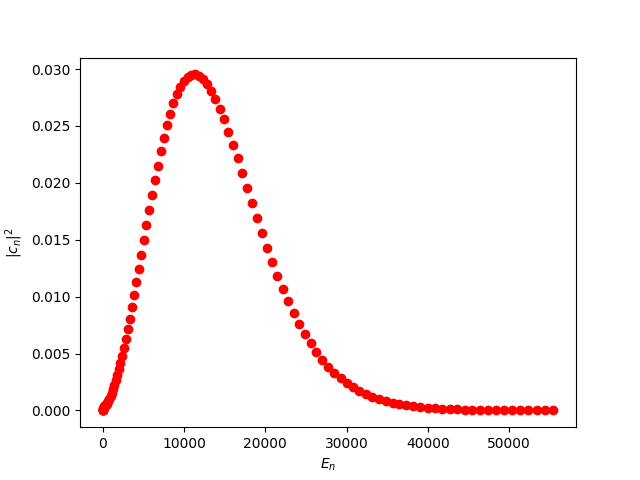
\includegraphics[width=\textwidth]{../Python/WiW_wavePackageEnergySpectrum.png}
\caption{Energy spectrum of the wave package in the finite square well} \label{fig:energySpectrumFinite}
\end{figure}

The energy spectra shown in figure~\ref{fig:energySpectrumInfinite} and figure~\ref{fig:energySpectrumFinite} show that our wave packages are in a superposition of stationary states which are eigenfunctions of the Hamiltonian. Thus if we were to measure the energy of one of our wave package we would only be able to measure the energies shown in the figures. It is important to note that we can only measure the discrete energies plotted and not any energy in between. When we measure the energy of one of our wave package $\abs{c_n}^2$ represents the probability of measuring a certain energy. Hence if we were to measure the energy of one of our wave package in the finite square well inside the infinite square well we would be more likely to observe energies around $10~000$ than energies around $40~000$ and we would never measure energies above $60~000$.

\section{Conclusion}
We have in this report seen how many of the peculiarities of quantum mechanics can be visualized through the use of numerics in the case of the relatively simple potentials of the infinite and finite square well. We have also seen how the numerics highlights some of the stranger features of the potentials which result from the potentials being idealizations of real world potentials.

\newpage
\appendix
\section{Appendix: Code Snippets}
This appendix includes some of the interesting excerpts from our code.
\subsection{Newton's Method} \label{app:newton}
We have implemented Newton's method in our script used for finding the allowed energy levels of the stationary states in the finite square well as follows:
\lstinputlisting[firstnumber=53,firstline=53,lastline=73]{../Python/FSW_psi_n_bound.py}
Here \lstinline{hfuns} is a previously defined list of functions which correspond to equations \eqref{eq:evenEnergy} and \eqref{eq:oddEnergy} with the RHS subtracted from the LHS. The derivatives \lstinline{dhdzfuns} are calculated symbolically since the numerical derivative was erroneous near the singularities of $\tan z$ and $\cot z$. As initial guesses we use values slightly below the singularities of $\tan z$ and $\cot z$ respectively.

\subsection{The Main Script}
This section will give a bit more detail on the main script in which we simulate the wave package.

\lstinputlisting[firstnumber=12,firstline=12,lastline=13]{../Python/wavePackageSimultaneousPlot.py}

Through experimenting with the code we have found that it is important to have a good resolution in the position array. Likewise we need a good resolution in the time array since the wave functions with higher energies have a small period. We simulate up until $t = \frac{4}{\pi}$ since this is the largest period of any of the wave functions and all the other wave functions have periods which divides this.

\lstinputlisting[firstnumber=15,firstline=15,lastline=32]{../Python/wavePackageSimultaneousPlot.py}

Before we compute the $c_n$'s we normalize the wave package using \lstinline{numpy.trapz} to determine the normalization constant. The default option for the \verb!getcn! module is to calculate $c_n$'s until the square norm of the $c_n$'s is below $10^{-12}$. Because the $c_n$'s have a square norm close to $1$ the integral of the wave function is also close to $1$. In the case of the infinite square well \lstinline{getcn} returns 48 $c_n$'s and the integral has a value of $0.99999999999907341$.

\lstinputlisting[firstnumber=41,firstline=41,lastline=43]{../Python/wavePackageSimultaneousPlot.py}

We calculate the wave function for all times to avoid extra function calls whenever we need the wave function. This saves us calculations when we calculate expected values, calculate the momentum spectrum and animate the wave function.

\lstinputlisting[firstnumber=45,firstline=45,lastline=66]{../Python/wavePackageSimultaneousPlot.py}

We calculate the expected values using the standard integrals. To determine $\pdiff{\Psi}{x}$ we use numerical differentiation with \lstinline{numpy.gradient}.

\lstinputlisting[firstnumber=70,firstline=70,lastline=82]{../Python/wavePackageSimultaneousPlot.py}
To calculate the momentum distribution we loop over the momentum array because we have to calculate an integral over position space for each point in the momentum spectrum.

The remainder of the code is about 60 to 70 lines of setting up, running and saving the animation. Please note that it can take a long time to encode a four to five minute video at near HD.

\end{document}
